\begin{figure}[!h]
%\vspace{-1pt} %takes away some white space before figure
\centering
\begin{subfigure}[b]{1.0\textwidth}
	\centering
	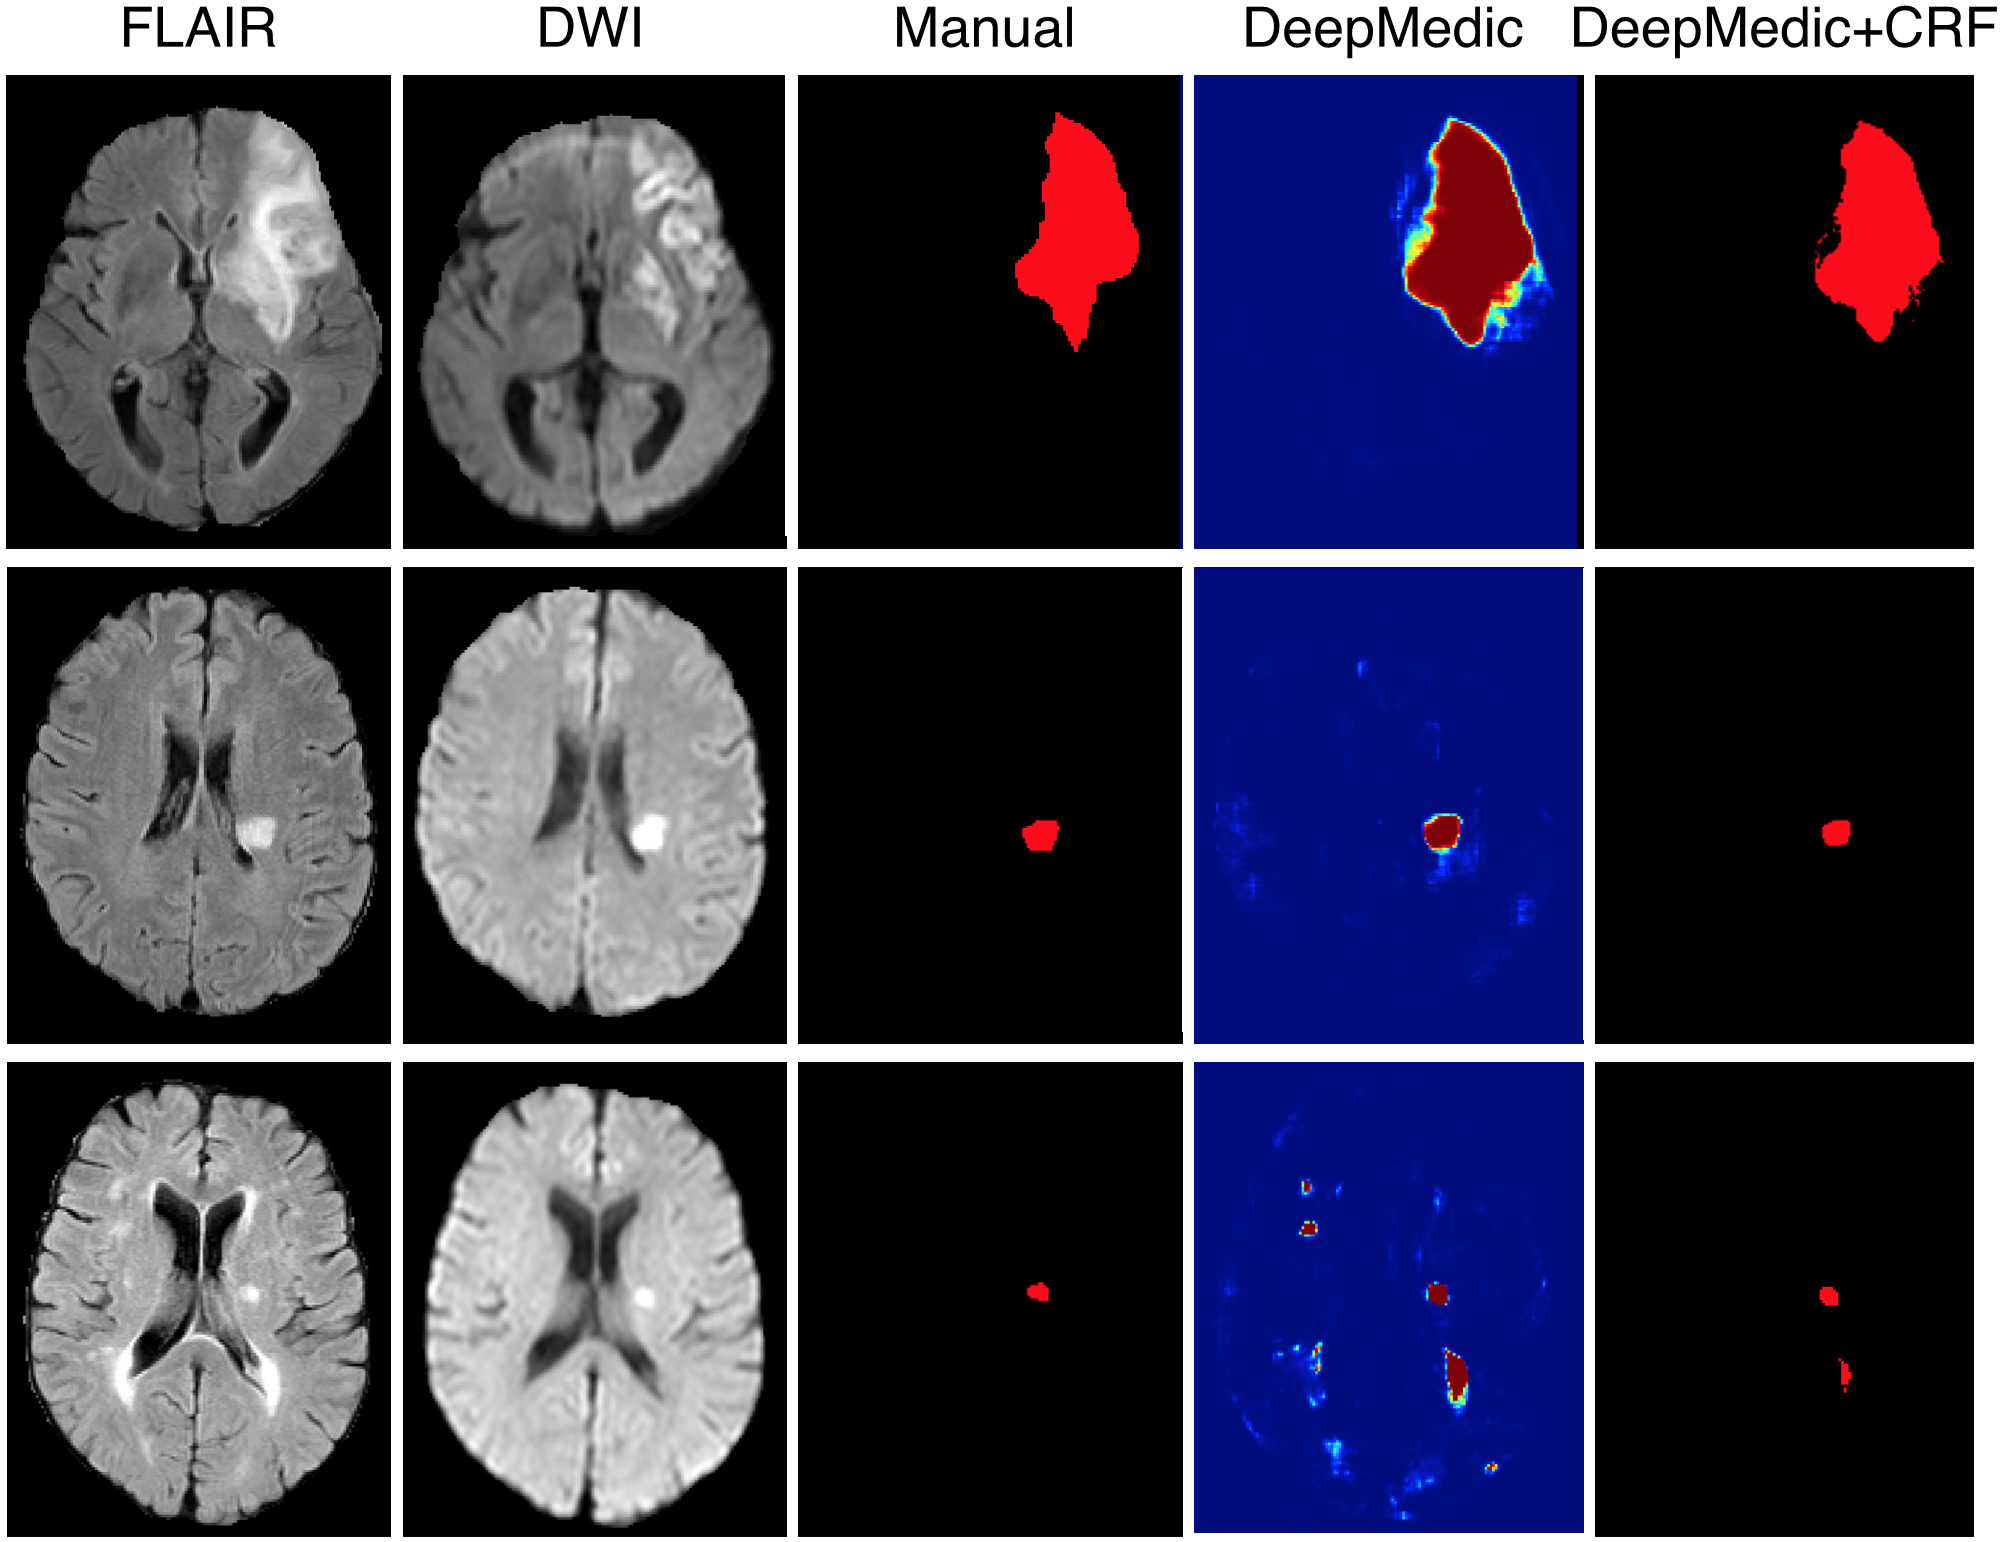
\includegraphics[clip=true, trim=0pt 0pt 0pt 0pt, width=1.0\textwidth]{figures/evaluationSection/isles/qualitative/isles15TrainingQualitatively.png}
\end{subfigure}
\vspace{-0pt} %takes away some white space before the caption
\caption{Examples of segmentations performed by our system on the training datasets of (SISS) ISLES 2015. (top and middle) The system is capable of satisfying segmentation of both large and smaller lesions. (bottom) Common mistakes are performed due to the challenge of differentiating stroke lesions from White Matter lesions. }
\label{fig:evalIslesVisualQuality}
\end{figure}
%\vspace{-1pt} %takes away some white space after figure